% !TeX document-id = {d7bfea81-c3f6-4000-b3a4-ebfa033e41d4}
% !TeX root = ./main.tex
% !TEX program = xelatex
% !BIB program = biber
% !TEX encoding = UTF-8 Unicode
% !TEX options = --shell-escape -synctex=1 -interaction=nonstopmode -file-line-error "%DOC%"
\documentclass{kuee_en}

% if your prefer Times New Roman in Windows, pleas uncomment the below two lines.
% \usepackage{fontspec}
% \setmainfont{Times New Roman}
% and comment these two line
\usepackage[T1]{fontenc}
\usepackage{mathptmx}

\usepackage{setspace}
% set line spacing here, if you want change the line number per page
\setstretch{1.2} % 36 lines per page
%\singlespacing % 43 lines per page
%\onehalfspacing % 33 line per page

% using modern biblatex
\bibliography{sample}

\title{An English \LaTeX{} Template for KUEE}
\etitle{An English \LaTeX{} Template for KUEE}
\eauthor{Denki Jiro} % english name, used in abstract page
\author{{電気 次郎}} % name shown in the cover, same as \eauthor if you don't have a kanji name 
\supervisor{{電気 太郎 教授}}
\school{{京都大学大学院工学研究科}}
\depart{{電子工学専攻}}
% \depart{{電気工学専攻}}
\date{{令和2年2月1日}}

\begin{document}
\maketitle

% abstract here
\begin{abstract}
    \lipsum[1]
\end{abstract}

% generate the contents
\tableofcontents

\chapter{How to use}

This template is designed for the english writer for master thesis in KUEE. All the formats are referred to the Japanese guide of master thesis\cite{tebiki}.
% \footnote{修士論文作成規定および手引, 2019年12月13日改定}
In the case of PhD students, it is free to use any \LaTeX ~template as I know in KUEE. For undergraduate students, I think only Japanese is acceptable. If necessary, it is easy to change the title name in \verb|kuee_en.cls|
\footnote{Hint, line 37}.

The default compiler of this template is \verb|xelatex| as magic commands are defined in this file head. This is due to the use of \verb|xeCJK| and \verb|fontspec| packages. If you want the old-fashioned \verb|pdflatex| or \verb|latex|, please note the package compatibility, which do not support the Japanese cover.

\section{Line spacing}
The required line number per page in Japanese version\cite{tebiki} is about 32. While default \verb|a4paper| using single spacing in \LaTeX, means more than 40 lines per page. Despite the language difference, 1.2 line spacing is recommended.

This value is adjustable in the macro of package \verb|setspace| if you like. 
Set the linespacing in the file head and then check the line number with the text in Chapter 2.

\section{CJK languages}

\verb|xeCJK| package is used in this paper to generate the cover page.
\begin{quote}
電気・電子工学は現代のあらゆる産業や社会生活の基盤として欠くことのできない科学技術となっています。例えば,大規模集積回路(超LSI)や光・半導体デバイスを用いた各種の電子・情報・通信システム,ホームエレクトロニクス機器,ロボット・自動車・通信衛星・医療福祉機器等に搭載されている人工知能や制御システムなどはその代表としてあげられます。また,現代社会の主要なエネルギー源である電力の高効率で安定な供給に関する技術とともに,あらゆる電気・電子応用機器の高効率化や人間社会・地球環境との調和のための技術がますます重要になってきています。
\end{quote}
Except quotation, it requires \{\} to insert Japanese characters inline, like
{電気・電子工学}. 
Note, this is also important for reference. Add \{\} for any Japanese item in \verb|.bib| file if you want to cite them.

The default font is Meicho font.
Please note the Meicho font is only for Japanese characters, it may not work for the specific characters from Korean and Chinese. 

\section{Formula for scientists}
The modern package \verb|physics| \footnote{See, http://mirrors.ibiblio.org/CTAN/macros/latex/contrib/physics/physics.pdf} is required in the style file.

Multiple-line aligned example, Maxwell Equations
\begin{align}
    \div{\vb{D}} &= 0 \\
    \div{\vb{B}} &= 0 \\
    \curl{\vb{E}} &= -\pdv{\vb{B}}{t} \\
    \curl{\vb{H}} &= \pdv{\vb{D}}{t}
\end{align}

Schr\"{o}edinger Equation
\begin{equation}
	i\hbar \pdv{\ket{\varphi}}{t} = \mathcal{H} \ket{\varphi}
\end{equation}

Chemical equation example
\begin{equation*}
    2\ce{H2}+\ce{O2} \longrightarrow 2\ce{H2O}
\end{equation*}

\section{References and citation}
The reference format is modified for the format required in KUEE based on the nature style defined in the \verb|nature-style.bbx|.  

Cite this paper \cite{Kiyohara2020}, cite again \cite{Okano2015}, and cite several ones together \cite{Nagata2007, Sugiura2019}.

\section{Figures and tables}
All the figures and tables are automatically floated to the file end. Here is an example. And the comes with appendices.

A tikz figure shown in Fig. \ref{fig:tikz}.

\begin{figure}
    \centering
    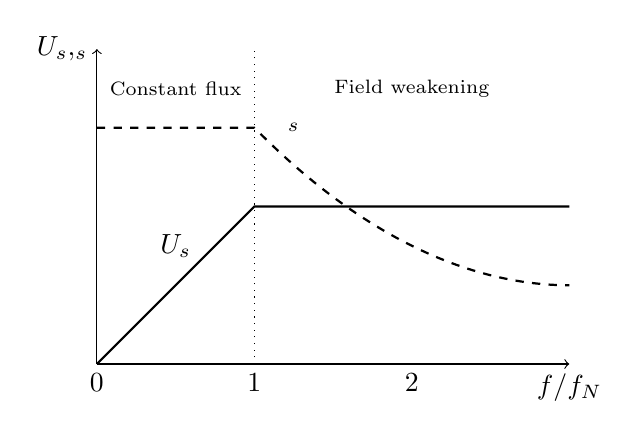
\begin{tikzpicture}
    % horizontal axis
    \draw[->] (0,0) -- (6,0) node[anchor=north] {$f/f_N$};
    % labels
    \draw	(0,0) node[anchor=north] {0}
    		(2,0) node[anchor=north] {1}
    		(4,0) node[anchor=north] {2};
    % ranges
    \draw	(1,3.5) node{{\scriptsize Constant flux}}
    		(4,3.5) node{{\scriptsize Field weakening}};
    % vertical axis
    \draw[->] (0,0) -- (0,4) node[anchor=east] {$U_s,\varPsi_s$};
    % nominal speed
    \draw[dotted] (2,0) -- (2,4);
    % Us
    \draw[thick] (0,0) -- (2,2) -- (6,2);
    \draw (1,1.5) node {$U_s$}; %label
    % Psis
    \draw[thick,dashed] (0,3) -- (2,3) parabola[bend at end] (6,1);
    \draw (2.5,3) node {$\varPsi_s$}; %label
    \end{tikzpicture}
  \caption{A tikz figure example}
  \label{fig:tikz}
\end{figure}

Default parameters used in this template is shown in Tab.\ref{tab:text}, Tab.\ref{tab:fig}.

\begin{table}
  \caption{Default layout}\label{tab:text}
  \begin{center}
    \begin{tabular}{|l|r|}
      \hline
      \verb+\textwidth+ & 424pt \\ \hline
      \verb+\textheight+ & 604pt \\ \hline
      \verb+\oddsidemargin+ & 0.5cm \\ \hline
      \verb+\evensidemargin+ & 0.5cm \\ \hline
      \verb+\topmargin+ & 0pt \\ \hline
      \verb+\headheight+ &12pt \\ \hline
      \verb+\headsep+ & 25pt \\ \hline
      \verb+\footskip+ & 30pt \\ \hline
    \end{tabular}
  \end{center}
\end{table}

\begin{table}
  \caption{Default parameters for graphs}\label{tab:fig}
  \begin{center}
    \begin{tabular}{|l|r|}
      \hline
      \verb+\textwidth+ & 424pt + 1cm \\ \hline
      \verb+\textheight+ & 604pt + 67pt \\ \hline
      \verb+\oddsidemargin+ & 0pt \\ \hline
      \verb+\evensidemargin+ & 0pt \\ \hline
      \verb+\topmargin+ & 0pt \\ \hline
      \verb+\headheight+ & 0pt \\ \hline
      \verb+\headsep+ & 0pt \\ \hline
      \verb+\footskip+ & 0pt \\ \hline
    \end{tabular}
  \end{center}
\end{table}


\chapter{Lorem Ipsum}
\lipsum[1-10]


\begin{acknowledgements}
\lipsum[2]
\end{acknowledgements}

\printbibliography[title=References,heading=bibintoc]

\clearpage % ensure all floats are processed
\processdelayedfloats
\clearpage

\begin{appendices}
\chapter{Versions}
\begin{description}
  \item[2019] 1st version by Zhenghao Yin, Takeuchi lab.
\end{description}
\end{appendices}


\end{document}

